\chapter{ម៉ាសុីន}
\section{លំនាំអាដ្យាបាទិច}
\begin{definition}
	លំនាំអាដ្យាបាទិច ជាលំនាំដែលថាមពលកម្តៅមិនប្តូរជាមួយមជ្ឈដ្ឋានក្រៅ(មិនស្រូប និងមិនបញ្ចេញកម្តៅ) ឬមានតម្លៃថេរជានិច្ច $\left(Q=0\right)$។ តាមច្បាប់ទីមួយទែម៉ូឌីណាមិចយើងបានៈ $W=-\Delta U$។
\end{definition}
\begin{example}
	\begin{enumerate}[m]
		\item កាលណាឧស្ម័នត្រូវបានបណ្ណែនតាមបែបអាដ្យាបាទិច កម្មន្តបានធ្វើទៅលើឧស្ម័ននោះគឺ $640J$។\\ គណនាបម្រែបម្រួលថាមពលក្នុងរបស់ឧស្ម័ន។
		\item ក្នុងប្រព័ន្ធត្រមោចមួយ បើថាមពលក្នុងថយចុះ $500J$ តើកម្មន្តដែលបំពេញដោយប្រព័ន្ធនោះស្មើនឹងប៉ុន្មាន?
	\end{enumerate}
\end{example}
\section{សុិចកាកណូ}
\subsection{សុិចកាកណូ}
\begin{definition}
	\emph{\kml សុិចកាកណូៈ} សុិចកាកណូជាលំនាំរេវែសុីប នៃម៉ាសុីនប្រើកម្តៅដែលផ្តូចផ្តើមគំនិតដោយលោក \emph{សាឌីកាណូ}។
\end{definition}
សុិចកាណូ មានបួនដំណាក់កាលៈ
	\begin{itemize}
		\item [$-$] \emph{\kml ដំណាក់កាលទី១ៈ​} ឧស្ម័នស្រូបកម្តៅតាមលំនាំអុីសូទែម។ ឧស្ម័នរីកមាឌ និងមានសម្ពាធថយចុះ។
		\item [$-$] \emph{\kml ដំណាក់កាលទី២ៈ} ឧស្ម័នបន្តរីកមាឌ និងថយចុះសម្ពាធតាមលំនាំអាដ្យាបាទិច។
		\item [$-$] \emph{\kml ដំណាក់កាលទី៣ៈ} ឧស្ម័នបញ្ចេញកម្តៅ ពិស្តុងធ្លាក់ចុះសង្កត់ឧស្ម័ន។ ឧស្ម័នរួមមាឌតាមលំនាំអុីសូទែម។
		\item [$-$] \emph{\kml ដំណាក់កាលទី៤ៈ} ឧស្ម័នត្រូវបានបណ្ណែនតាមលំនាំអាដ្យាបាទិចរហូតដល់ភាពដើមវិញ។
	\end{itemize}
	\begin{figure}[H]
		\centering
		\begin{tikzpicture}[
		> = latex,
		dot/.style = {draw,fill,circle,inner sep=1pt},
		arrow inside/.style = {postaction=decorate,decoration={markings,mark=at position .55 with \arrow{>}}}
		]
		\begin{scope}
		\draw[<->] (0,4.5) node[left] {$P$} |- (4.5,0) node[right] {$V$};
		\node[dot,label={above:$a$}] (@a) at (0.5,4) {};
		\node[dot,label={right:$b$}] (@b) at (2.5,3) {};
		\node[dot,label={right:$c$}] (@c) at (4,1) {};
		\node[dot,label={below:$d$}] (@d) at (1.5,2) {};
		\draw[arrow inside] (@a) to[looseness=.7,bend right=20] (@b);
		\draw[arrow inside] (@b) to[looseness=.7,bend right=20] (@c);
		\draw[arrow inside] (@c) to[looseness=.7,bend left=20] (@d);
		\draw[arrow inside] (@d) to[looseness=.7,bend left=20] (@a);
		\draw[->, line width=3pt] (2,3.5) -- (2,2.5);
		\draw[->, line width=3pt] (2,2) -- (2,1);
		\node[label={above:$Q_{h}$}] at (2,3.5) {};
		\node[label={below:$Q_{c}$}] at (2,1) {};
		
		\node [cylinder,cylinder uses custom fill, cylinder end fill=yellow!20,
		cylinder body fill=cyan!15!white, shape border rotate=90, minimum width=2cm, minimum
		height=2.8cm, aspect=2.5, overlay, draw] {};
		\draw[opacity=0.25] (-1,-.8) arc (180:0:1cm and 0.5cm);
		\fill[gray] (0,-.72) circle [x radius=.9cm, y radius=0.35cm];
		\draw (0,0) node {$P_{i}$};
		\end{scope}
		\end{tikzpicture}
	\end{figure}
\begin{figure}[H]
	\centering
	\begin{tikzpicture}
	\def\lmag{1.8}  % length of magnet
	\def\wmag{0.4}  % thickness of magnet
	\def\nc{5}      % number of lines = 2*\nc+1
	
	\begin{scope}
	\coordinate (A) at (-\lmag/2,\wmag/2);
	\coordinate (B) at (\lmag/2,-\wmag/2);
	\draw[fill, color=blue](A) rectangle ++(\lmag/2,-\wmag)node[white,midway]{S};
	\draw[fill, color=red](0,-\wmag/2) rectangle ++(\lmag/2,\wmag)node[white,midway]{N};
	
	\clip (-5,-3) rectangle (5,3);
	\foreach \r in {1,...,\nc}{
		\draw[fLines]($(A)-(0,0.5*\r*\wmag/\nc)$) arc(({270-asin(\lmag/(2*\r))}):({-90+asin(\lmag/(2*\r))}):\r);
		\draw[fLines]($(B)+(0,0.5*\r*\wmag/\nc)$) arc(({90-asin(\lmag/(2*\r))}):({-270+asin(\lmag/(2*\r))}):\r); }
	\draw[fLines] (-\lmag/2,0) -- ++(-6,0);
	\draw[fLines] (\lmag/2,0) ++(6,0)--(\lmag/2,0);
	\end{scope}
	\end{tikzpicture}
	\caption{ខ្សែដែនជុំវិញរបារមេដែក}
\end{figure}
\begin{figure}[H]
	\centering
	\begin{tikzpicture}[scale=1.8]
	\draw[<->] (3,0) node[below] {$V$} -| (0,2.5) node[left] {$P$};
	\path (1,1) coordinate (2) {} (2.5,.8) coordinate (1) {}
	(1,2) coordinate (3) {} (2.5,1.5) coordinate (4) {};
	\path[font=\footnotesize] (1) node[below right] {1}
	(2) node[left] {2}
	(3) node[above right] {3}
	(4) node[above right] {4};
	\draw[mypath=.4,shorten <=-.15cm] (1) to[bend left=5] (2);
	\path (x) node[below] {$\Delta Q=0$};
	\draw[mypath=.4,shorten <=-.2cm,shorten >=-.2cm] (3) to[bend right=15] (4);
	\path (x) node[above right] {$\Delta Q=0$};
	\draw[mypath=.5] (2) -- (3);
	\draw[->] (x)++(-.5,0) -- + (.3,0) node[midway,above] {$\Delta Q_h$};
	\draw[mypath=.5] (4) -- (1);
	\draw[<-] (x)++(.5,0) -- + (-.3,0) node[midway,above] {$\Delta Q_c$};
	\draw[dashed] (2) -- (1,0) node[below] {$V_2$}
	(1) -- (2.5,0) node[below] {$V_1$};
	\foreach \i in {1,...,4} \filldraw[fill=white] (\i) circle (1pt);
	\end{tikzpicture}
\end{figure}

\begin{figure}[H]
	\centering
	\begin{tikzpicture}[>={Triangle[angle=60:1 2]}, scale=1.5]
	\path [shading=heat]
	(-2,2) rectangle (2,3/2) (-2,-2) rectangle (2,-3/2);
	\draw (-2,3/2) -- (2,3/2) (-2,-3/2) -- (2,-3/2);
	\scoped{
		\clip (-3/2,-7/4) rectangle (3/2,7/4);
		\draw [shading=heat] 
		(3/4,2) -- (-3/4,2) -- (-3/4,7/4) arc (90:0:1/4) -- (-1/2,-3/2)
		arc (360:270:1/4) -- (-3/4,-2) -- (1/4,-2) -- (1/4,-7/4) 
		arc (270:180:1/4) -- (0,-3/2)    -- (0,1/4)   
		arc (180:270:1/2) -- (2,-1/4)  -- (2,1/4) -- (3/4,1/4)
		arc (270:180:1/4) -- (1/2,3/2)  arc (180:90:1/4) -- (3/4,2);
	}
	\path (0,2.6) node {\text{ធុងក្តៅ} $T_h$} (0,-2.5) node {\text{ធុងត្រជាក់} $T_c$} (0,2) node {$Q_{h}$} (-.2,-1.8) node {$Q_{c}$} (3.5,0) node {$W=\abs{Q_{h}}-\abs{Q_{c}}$} (2.7,1) node {\text{ម៉ាសុីន}};
	\draw [red!75,  line width=1cm/4, ->] (0,3/2) -- (0,1/2);
	\draw [red!75,  line width=1cm/8, ->] (-1/4,-1/2) -- (-1/4,-3/2);
	\draw [blue!75, line width=1cm/8, ->] (1,0) -- (2,0);
	\draw (0,.2) circle (.8cm);
	\draw[->, line width=2pt] (2,1) -- (.7,.8);
	\end{tikzpicture}
	\caption{គំនូសតាងការបម្លែងថាមពលកម្តៅ}
\end{figure}
\begin{figure}[H]
	\centering
	\begin{tikzpicture}[tangent of circles/.style args={% https://tex.stackexchange.com/a/464143/194703
		at #1 and #2 with radii #3 and #4}{insert path={%
			let \p1=($(#2)-(#1)$),\n1={atan2(\y1,\x1)},\n2={veclen(\y1,\x1)*1pt/1cm},
			\n3={atan2(#4-#3,\n2)}
			in ($(#1)+(\n3+\n1+90:#3)$) coordinate(aux1) -- 
			($(#2)+(\n3+\n1+90:#4)$) coordinate(aux2)}},
	pics/engine/.style={code={
			\tikzset{engine/.cd,#1}
			\draw[fill=gray!20] (0,0) -- (-0.8,-0.4) coordinate[pos=0.4] (p1)
			coordinate[pos=0.8] (p2) |- (-1,-3)[rounded corners=1mm] |- (-1.2,0) [sharp corners]
			-- (-1.2,0.7) coordinate[pos=0.2] (p3)
			coordinate[pos=0.8] (p4) -- (-0.9,0.85) -- (-0.6,0.7) -- (0,0.4) -- (0.6,0.7)
			-- (0.9,0.85)-- (1.2,0.7) -- (1.2,0)coordinate[pos=0.2] (p6)
			coordinate[pos=0.8] (p5) {[rounded corners=1mm] -- (1,0)}
			[sharp corners] -- (1,-3)
			-| (0.8,-0.4) -- cycle coordinate[pos=0.2] (p8)
			coordinate[pos=0.6] (p7);
			\draw[engine/left exhaust] (p1) to[bend right=18] (p4) -- (p3) to[bend left=18] (p2) -- cycle;
			\draw[engine/right exhaust] (p7) to[bend left=18] (p6) -- (p5) to[bend right=18] (p8) -- cycle;
			\draw[fill=gray!50] (0,-4) circle[radius=4mm];
			\pgfmathsetmacro{\pistonpos}{-4+0.4*sin(\pgfkeysvalueof{/tikz/engine/rod angle})
				+sqrt(1.5*1.5-pow(0.4*cos(\pgfkeysvalueof{/tikz/engine/rod angle}),2))}
			\path (0,-4) + (\pgfkeysvalueof{/tikz/engine/rod angle}:0.4) coordinate (p9)
			(0,\pistonpos) coordinate (p10);
			\draw[fill=gray!15] (p9) circle [radius=2mm] -- (p10) circle [radius=1mm];
			\path[tangent of circles={at p10 and p9 with radii 0.1 and 0.2}]
			(aux1) coordinate (aux3) (aux2) coordinate (aux4); 
			\path[tangent of circles={at p9 and p10 with radii 0.2 and 0.1}];
			\path[fill=gray!15] (aux1) -- (aux2) -- (aux3) -- (aux4);
			\draw  (aux1) -- (aux2)  (aux3) -- (aux4);
			\path[fill=gray!45] (p9) circle [radius=1.2mm];
			\draw[left color=gray!40,right color=gray!20,middle color=white] (-0.8,\pistonpos) 
			rectangle ++ (1.6,1);
			\draw[left color=\pgfkeysvalueof{/tikz/engine/interior color}!40,
			right color=\pgfkeysvalueof{/tikz/engine/interior color}!20,
			middle color=white] 
			(-0.8,\pistonpos+1) --  (-0.8,-0.4)  -- (0,0)--  (0.8,-0.4) |- cycle;
			\draw[thin,fill=gray!30] (-0.42,-0.5) 
			++ ({90+atan(1/2)}:\pgfkeysvalueof{/tikz/engine/left valve}) 
			-- ++ ({90+atan(1/2)}:1.9) -- ++ ({atan(1/2)}:0.1)
			-- ++ ({-90+atan(1/2)}:1.9) -- ++({atan(1/2)}:0.3)
			-- ++ ({-90+atan(1/2)}:0.1) -- ++({atan(1/2)+180}:0.7)
			-- ++ ({90+atan(1/2)}:0.1) -- cycle;
			\draw[thin,fill=gray!30] (0.42,-0.5) 
			++ ({90-atan(1/2)}:\pgfkeysvalueof{/tikz/engine/right valve}) 
			-- ++ ({90-atan(1/2)}:1.9) -- ++ ({180-atan(1/2)}:0.1)
			-- ++ ({-90-atan(1/2)}:1.9) -- ++({180-atan(1/2)}:0.3)
			-- ++ ({-90-atan(1/2)}:0.1) -- ++({-atan(1/2)}:0.7)
			-- ++ ({90-atan(1/2)}:0.1) -- cycle;
	}},engine/.cd,left valve/.initial=0,right valve/.initial=0,
	left exhaust/.style={fill=gray!50},
	right exhaust/.style={fill=gray!50},
	rod angle/.initial=30,interior color/.initial=white] 
	\path (0,0) pic{engine={right valve=0.25,rod angle=0}} (5,0) pic{engine={left valve=0.25,rod angle=180}};
	\end{tikzpicture}
\end{figure}
\begin{figure}[H]
	\centering
	\begin{tikzpicture}{>=Triangle[angle=60:.5cm 1]}
		\begin{scope}[draw={rgb:red,1;green,2;blue,5}, fill={black!30!green},line width=2.5pt]
			%\draw (0,0) -- (2,1);
			%\draw (0,0) -| (2,2);
			%\draw (0,0) |- (2,2);
			%\draw [<->] (3,0) -| (0,3);
			%\draw (0,2) .. controls (3,0) .. (2,2);
			%\fill[color=black!30!green] (0,2) .. controls (3,0) .. (2,2);
			%\filldraw[draw={rgb:red,1;green,2;blue,5}, fill={black!30!green}] (0,2) .. controls (3,0) .. (2,2);
			%\draw (0,2) .. controls (3,0) and (-1,0) .. (2,2);
			%\fill (0,2) .. controls (3,0) and (-1,0) .. (2,2);
			%\filldraw (0,2) .. controls (3,0) and (-1,0) .. (2,2);
			%\draw (0,0) rectangle (3,2);
			%\fill (0,0) rectangle (3,2);
			%\filldraw (0,0) rectangle (3,2);
			%\draw[fill, color=red] (0,0) rectangle (1.5,.8) node[white, midway]{$\mathbf{S}$};
			%\draw[fill, color=blue] (1.5,0) rectangle (3,.8) node[white, midway]{$\mathbf{N}$};
			%\draw[pattern=north west lines] (0,0) rectangle (1.5,.8) node[black, midway]{$\mathbf{S}$};
			%\draw[fill, color=blue] (1.5,0) rectangle (3,.8) node[white, midway]{$\mathbf{N}$};
			%\draw[pattern=north east lines] (1,1) circle (1cm);
%			\fill (1,1) circle (1cm);
			%\filldraw (1,1) circle (1cm);
			%\shade[shading=ball] (1,1) circle (1cm);
			%\shade[ball color=green] (1,1) circle (1cm);
			%\shadedraw[right color=red] (1,1) circle (1cm);
			%\shadedraw[left color=red] (1,1) circle (1cm);
			%\shade[bottom color=green!50!blue] (1,1) rectangle (3,2);
			%Ballon
%			\tikzstyle{balloon}=[ball color=green];    
%			\shade[balloon] ellipse (1.75 and 2);
%			\shade[balloon] (-.1,-2) -- (-.3,-2.2) -- (.3,-2.2) -- (.1,-2) -- cycle;
%			\draw (0,-2.2) -- (0,-5);
		\end{scope}
	\end{tikzpicture}
		\begin{tikzpicture}[>=stealth, shape aspect=.5]
		\draw[pattern=crosshatch dots] (0,-1.1) circle [x radius=1.1cm, y radius=0.29cm];
		\node [cylinder,cylinder uses custom fill, cylinder end fill=yellow!20,
		cylinder body fill=cyan!10, shape border rotate=90, minimum width=2cm, minimum
		height=3cm, aspect=2.5, overlay, draw] {};
		\end{tikzpicture}
		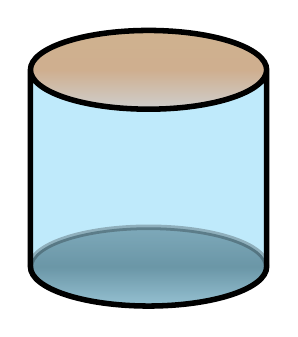
\begin{tikzpicture}[line width = 2pt]
		\fill[top color=gray!80!black,bottom color=black!10,middle color=black,shading=axis,opacity=0.25] (0,0) circle (1.5cm and 0.5cm);
		\fill[color=cyan,opacity=0.25] (1.5,0) -- (1.5,2.5) arc (360:180:1.5cm and 0.5cm) -- (-1.5,0) arc (180:360:1.5cm and 0.5cm);
		\fill[top color=orange!90!yellow,bottom color=orange!2,middle color=orange ,shading=axis,opacity=0.25] (0,2.5) circle (1.5cm and 0.5cm);
		\draw (-1.5,2.5) -- (-1.5,0) arc (180:360:1.5cm and 0.5cm) -- (1.5,2.5) ++ (-1.5,0) circle (1.5cm and 0.5cm);
		\draw[opacity=0.25] (-1.5,0) arc (180:0:1.5cm and 0.5cm);
		\end{tikzpicture}
\end{figure}

\begin{figure}[H]
	\centering
	
\begin{tikzpicture}
		\begin{scope}
			\draw [line width=2pt] (1,1) -- (2,2);
		\end{scope}
	\end{tikzpicture}
\end{figure}